%\begin{figure*}[t]
%\centering
%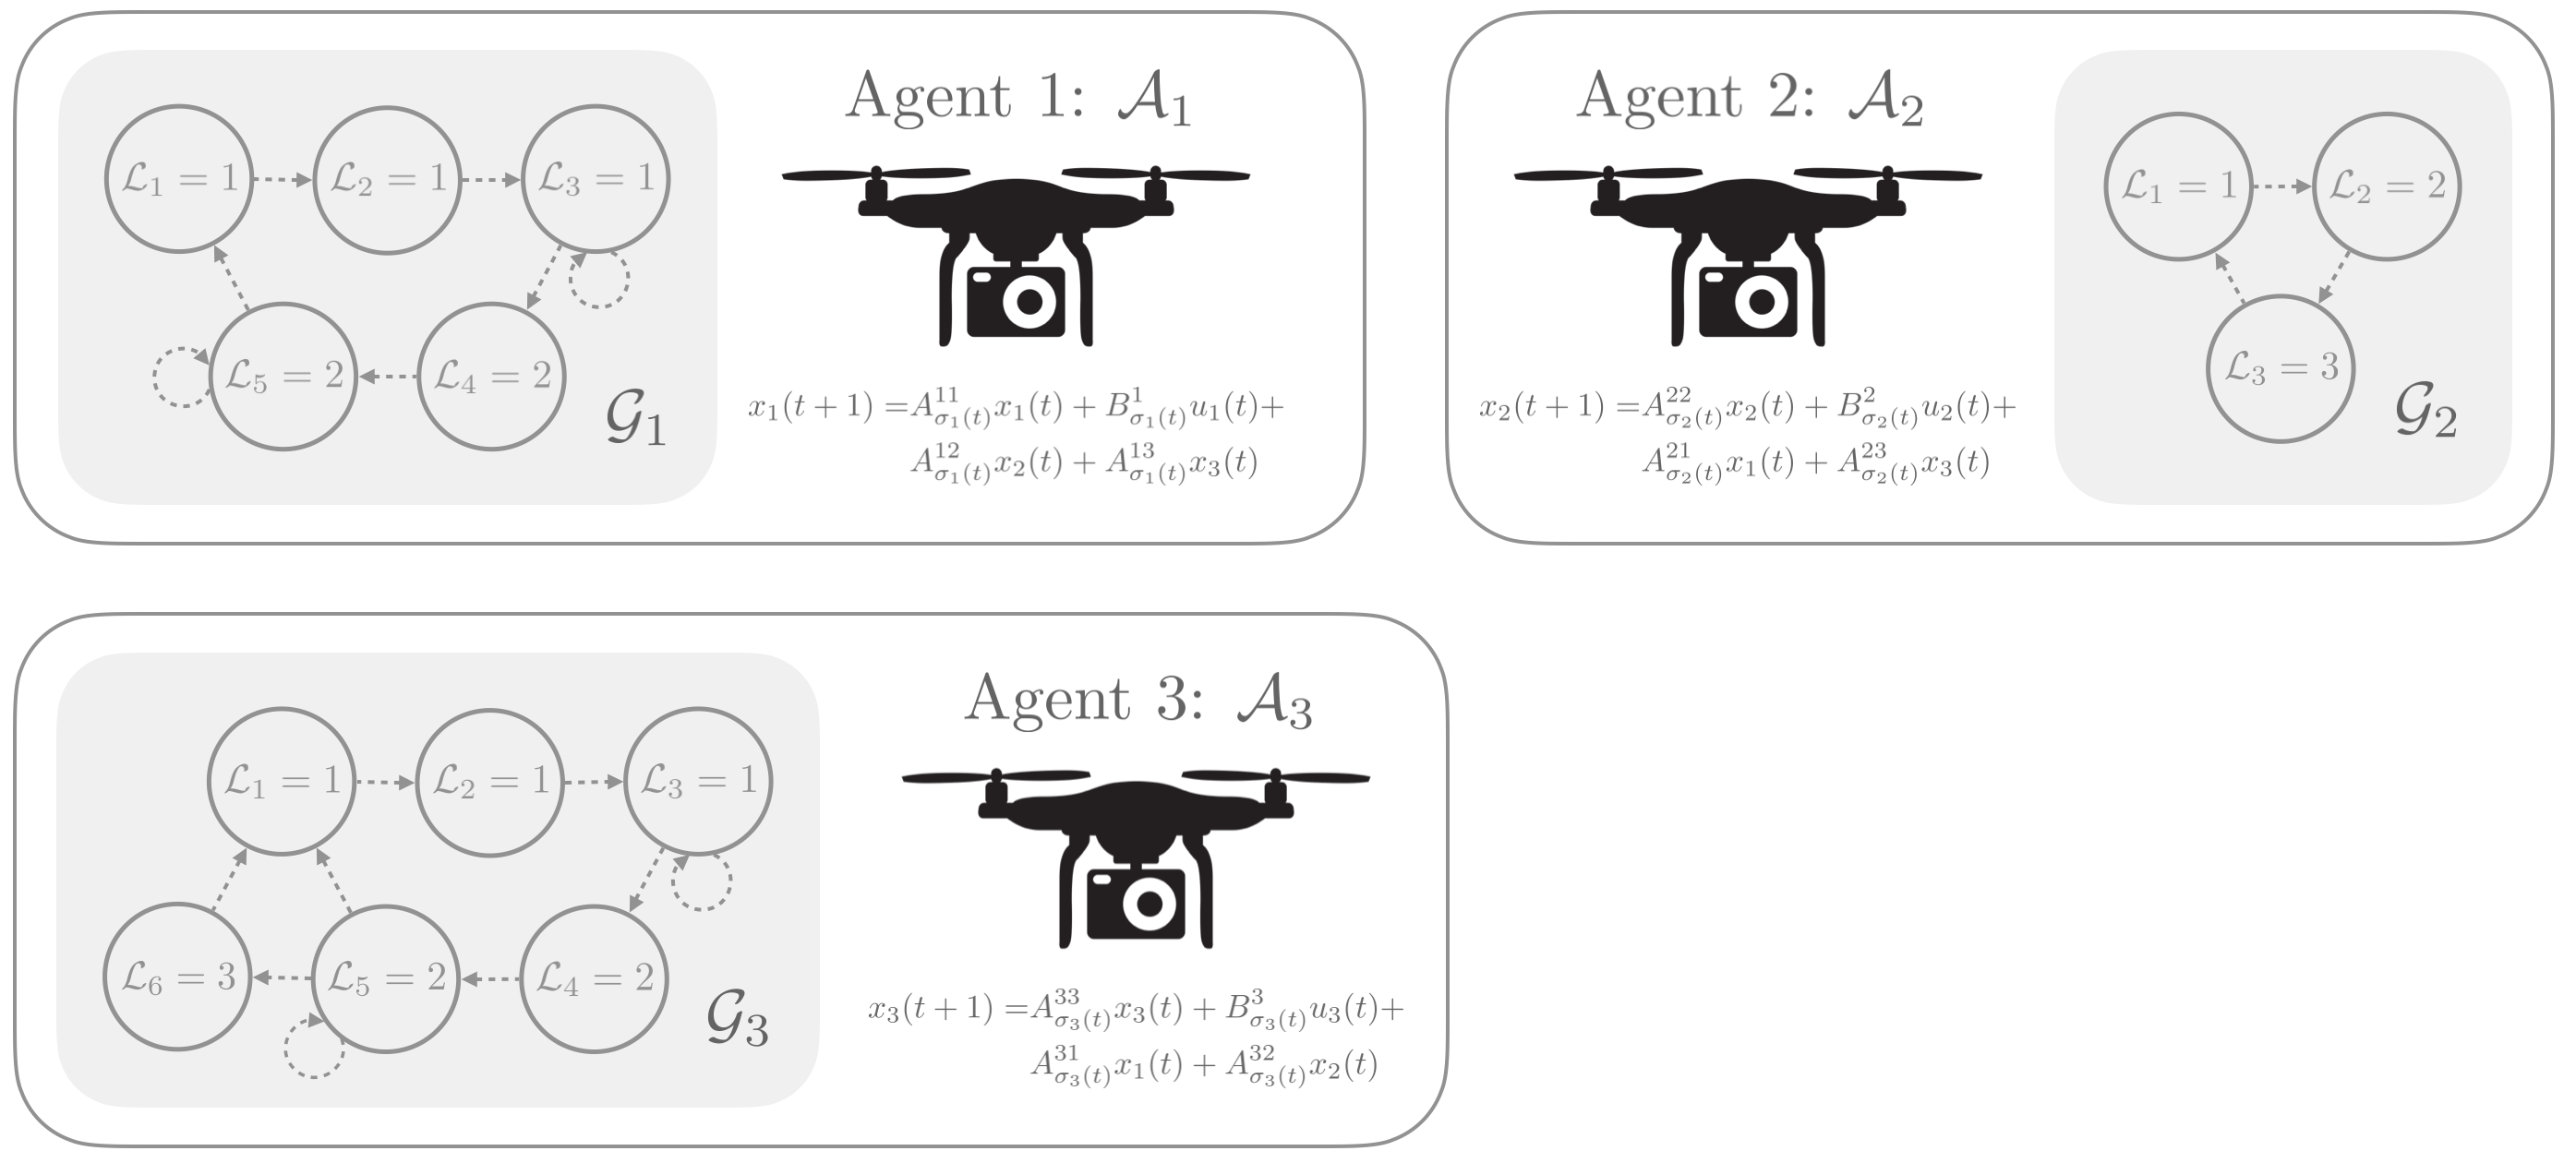
\includegraphics[width=\textwidth]{./figures/sample_system}
%\end{figure*}

\section{System Description}
In the previous \edit{sections}{section}, the systems have only contained a single switching signal. In general, however, switching signals may come from independent sources and merging them into a single signal would \edit{be less}{not be} justified. 

\edit{Consider a collection of $\numagents\in\int\rgeq{1}$ external switching signals each respecting their own directed graph, $\ss_\agentidx(t)\in\Sigma(\graph^\agentidx)\ \agentidx\in\idxset{\numagents}$. Further, consider a system with all of these signals and dynamics taking the form}{Consider a linear system partitioned into $\numagents$ agents where agent $\agentidx\in\idxset{\numagents}$ has states $x_\agentidx(\cdot)\in\real^{n_x^\alpha}$ and inputs $u_\agentidx(\cdot)\in\real^{n_u^\alpha}$. Each agent switches according to the local switching signal, $\ss_\agentidx(t)\in\Sigma(\graph^\agentidx),\ \agentidx\in\idxset{\numagents}$. These dynamics can be represented centrally as}
\begin{subequations}
\label{eq:sys}
\begin{align}
A(t)&=\begin{bmatrix}
A^{11}_{\ssl[1](t)}&A^{12}_{\ssl[1](t)}&\cdots&A^{1\numagents}_{\ssl[1](t)},\\
A^{21}_{\ssl[2](t)}&A^{22}_{\ssl[2](t)}&\cdots&A^{2\numagents}_{\ssl[2](t)},\\
\vdots&\vdots & \ddots & \vdots\\
A^{\numagents 1}_{\ssl[\numagents](t)} & A^{\numagents 2}_{\ssl[\numagents](t)} &\cdots & A^{\numagents \numagents}_{\ssl[\numagents](t)} 
\end{bmatrix},\label{eq:sys_A}\\
B(t)&=\begin{bmatrix}
B^{1}_{\ssl[1](t)} & \cdots & 0\\
\vdots             & \ddots & \vdots\\
0                  & \cdots & B^{\numagents}_{\ssl[\numagents](t)}
\end{bmatrix},\label{eq:sys_B}\\
\xcon(t)&=\xcon[\ssl[1](t)]^1\times\cdots\times\xcon[\ssl[\numagents](t)]^\numagents,\label{eq:sys_X}\\
\ucon(t)&=\ucon[\ssl[1](t)]^1\times\cdots\times\ucon[\ssl[\numagents](t)]^\numagents\label{eq:sys_Y}.
\end{align}
\end{subequations}
This structure is motivated by distributed systems with coupling in the system's states. Note how each block-row is governed by a single switching signal. This makes intuitive sense because local switching signals are more likely to effect how neighboring states impact the local agent rather then how local states will effect neighboring agents.

The goal of this work is to design a safe-set collection for systems with the above structure. \edit{A single signal could amalgamate all the individual switching signals. The definition of safe-sets, however, clearly shows that the exponential growth in the number of graph nodes corresponds to is an exponential growth in the cardinality of the safe-set collection.}{One possible solution could be to amalgamate the individual switching signals into a single signal and treat the system as centralized. This would cast the problem in the form of \autoref{eq:basic_switched_sys} and previous results could be used to compute a safe-set collection for the system \cite{Danielson2019}. However, this would lead to exponential growth in the number of nodes in the switching signal's graph matched by growth in the elements of the safe-set collection.}  This is computationally untenable. This is further exasperated in the high dimension systems with the block-row structure would tend to have. Having even just three block-rows each in $\real^3$ leads to a nine-dimensional system and will tax this naive implementation. These concerns will be addressed by splitting the system into block-rows and looking for safe-set collections, $\mathcal{S}^{\agentidx}=\{\mathcal{S}^\agentidx_n\}_{n\in\gnumnodes[\agentidx]}$, for each separately. Once found, the collections can be merged into a large collection with all possible switching signal states represented.

Looking only at the block row indexed by $\agentidx$, the dynamics can be rewritten as 
\edit{
\begin{align}
x_\agentidx(t+1)&=A^{\agentidx\agentidx}_{\ssl[\agentidx](t)}x_\agentidx(t)+B^\agentidx_{\ssl[\agentidx](t)}u_\agentidx(t)\nonumber\\&\quad+\sum_{\tilde\agentidx\in\idxset{\numagents}\setminus \agentidx}A^{\agentidx\tilde\agentidx}_{\ssl[\agentidx](t)}x_{\tilde\agentidx}(t)\\
&=A^{\agentidx}_{\ssl[\agentidx](t)}x_\agentidx(t)+B^\agentidx_{\ssl[\agentidx](t)}u_\agentidx(t)+E_{\ssl[\agentidx](t)}^\agentidx w(t),\nonumber
\end{align}
with $w(t)\in\wcon[\ssl[\agentidx](t)]^\agentidx$.}{\begin{align}\label{eq:block-row-dyn}
x_\agentidx(t+1)&=A^{\agentidx}_{\ssl[\agentidx](t)}x_\agentidx(t)+B^\agentidx_{\ssl[\agentidx](t)}u_\agentidx(t)+E_{\ssl[\agentidx](t)}^\agentidx w(t)
\end{align}
where
\begin{align*}
E_{\ssl[\agentidx](t)}^\agentidx =\left[A^{\agentidx\tilde\agentidx}_{\ssl[\agentidx](t)}\right]_{\tilde\agentidx\in\idxset{\numagents}\setminus \agentidx}\in\real^{n_x^\agentidx \times \sum_{\tilde\agentidx\in\idxset{\numagents}\setminus \agentidx} n_x^{\tilde\agentidx}}
\end{align*}
and $w(t)\in\wcon[\ssl[\agentidx](t)]^\agentidx\subset \real^{ \sum_{\tilde\agentidx\in\idxset{\numagents}\setminus \agentidx} n_x^{\tilde\agentidx}}$.}
 The existence of $\wcon[\ssl[\agentidx](t)]^\agentidx$ can be inferred from the fact that the full system is constrained. These dynamics and constraints are collected into the following tuple defining agent $\agentidx$,
$$\agent{\agentidx}\triangleq\{\{A^{\agentidx}_{\modeidx},B^\agentidx_{\modeidx}, E_{\modeidx}^\agentidx,\xcon[\modeidx]^\agentidx,\ucon[\modeidx]^\agentidx, \wcon[\modeidx]^\agentidx\}_{\modeidx=1}^{\nummodes[\agentidx]},\graph^\agentidx\}.$$
These can be collected into the full system
\begin{equation}\label{eq:agent_notation}
\agents\triangleq\{\agent{\agentidx}\}_{\agentidx\in\idxset{\numagents}}.
\end{equation}
Each agent only has a single switching signal explicitly appearing, $\ss_\agentidx(t)$, and resembles a locally switched system with additive disturbances. Previous, robust switched techniques, such as those developed in \cite{Lavaei2021}, may seem like possible solutions. However, $\wcon[\modeidx]^\agentidx$ is unknown. Though it can be characterized using the full state constraints, this would lead to conservative results because the actual safe-sets are, by definition, subsets of the state constraints. Alternatively, each of the neighboring agents could share its current safe-set. This however, returns the system to the centralized problem with its associated drawbacks. Furthermore, if \autoref{eq:block-row-dyn} represents a distributed system, this level of communication may be undesirable. Balancing these considerations, this work bounds the states of any given neighbor within the convex hull of the union of that neighbor's safe-set collection. This only requires acquiring a single set and relies on the state of the local switching signal alone. 